\section{Research Methodology}

\subsection{Overall Framework}

Fig.~\ref{fig:framework} summarises the pipeline: raw taxpayer data $\rightarrow$ preprocessing $\rightarrow$ feature engineering $\rightarrow$ Stage 1 segmentation $\rightarrow$ peer-group formation $\rightarrow$ Stage 2 Isolation Forest within each peer group $\rightarrow$ Stage 3 supervised classification $\rightarrow$ Stage 4 SHAP $\rightarrow$ risk interpretation and visualisation. Segmentation precedes anomaly detection because the reference population must be fixed before ``unusual'' can be defined: a forest fitted to the whole population isolates whatever is globally rare, whereas a forest fitted within a peer group isolates what is rare among similar taxpayers. The SHAP explainability describes both segment and anomaly score into which feature have mostly contributed to anomaly.

\begin{figure}[H]
    \centering
    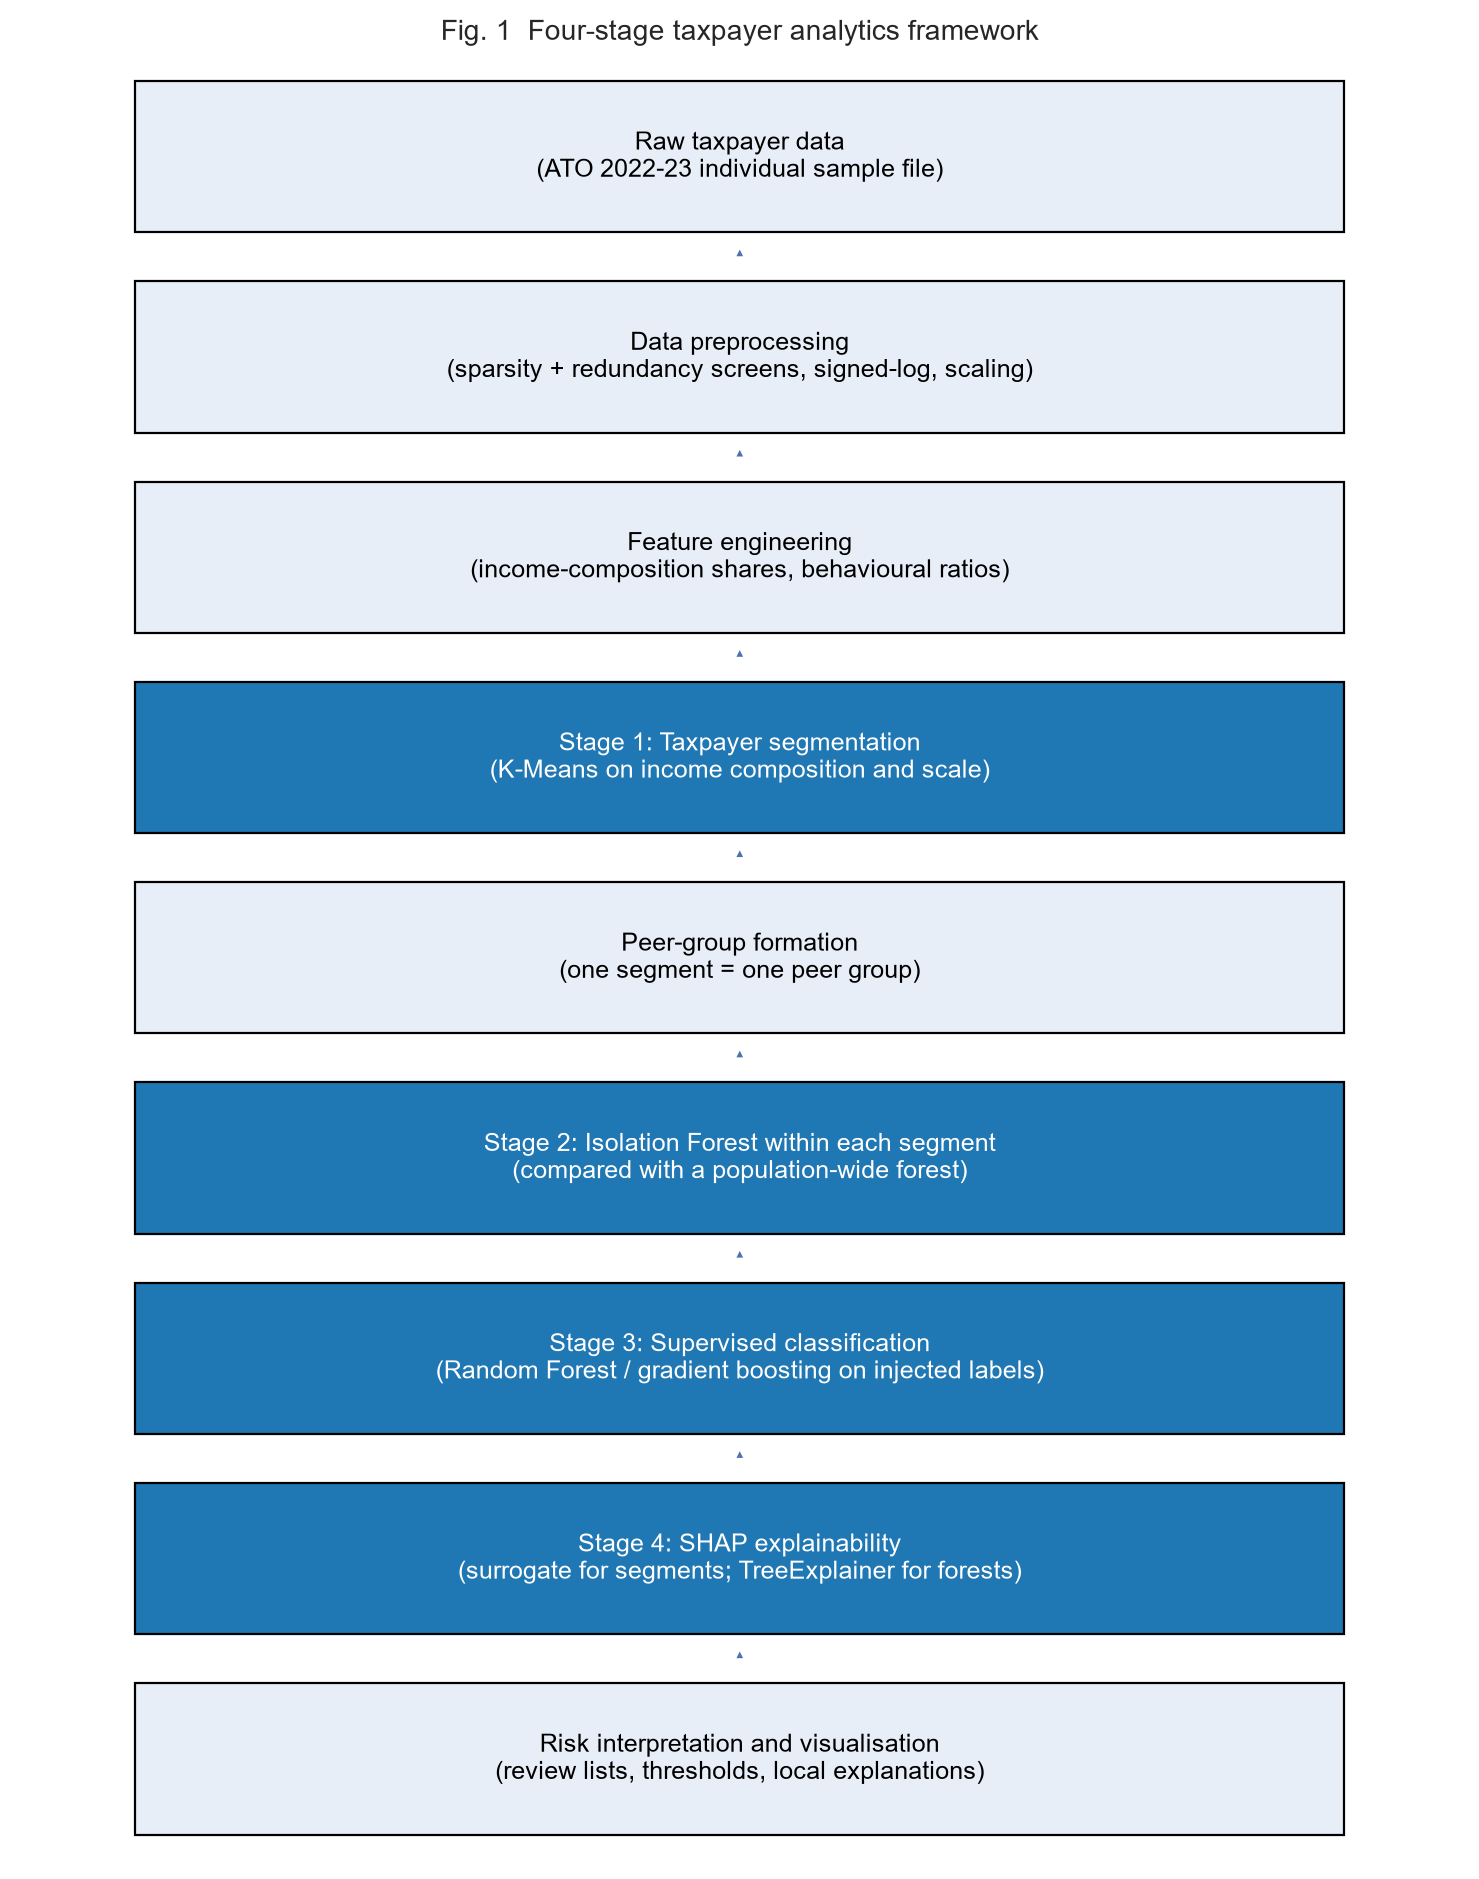
\includegraphics[width=0.6\linewidth]{figures/fig01_framework.png}
    \caption{Four-stage taxpayer analytics framework.}
    \label{fig:framework}
\end{figure}

\subsection{Dataset}

The primary data used in this research were obtained from Australian Taxation Authority and it covers the tax filing records of 2\% confidentialised random sample for Financial Year 2022 to 2023. It covers around 321,890 anonymised individual income tax returns data released by ATO only for research purposes. The access to the data is limited to the people who have signed Confidentiality Deed with ATO and granted through the ATO's taxation statistics program. The variable index for these data have sixty-five fields including taxpayer demographics, reported income, claimed deductions, offsets and etc. It has no personal information, such as name, address, DOB, or postcode. These variables group into below summarised groups in Table~\ref{tab:dataset}:

\begin{table}[H]
    \centering
    \caption{Dataset and preprocessing summary.}
    \label{tab:dataset}
    \begin{tabular}{ll}
        \toprule
        Characteristic & Value \\
        \midrule
        Source & ATO 2022--23 individual sample file (SA4 geography) \\
        Reference population & 16,108,843 individual taxpayers \\
        Records in the sample & 321,890 \\
        Sampling fraction & 1.9982\% \\
        Variables in the file & 65 \\
        Missing (blank) cells & 0 \\
        Fully duplicated records & 0 \\
        Financial variables available & 57 \\
        \bottomrule
    \end{tabular}
\end{table}

The data has sixty five variables belonging to several groups. Seven of them belongs to taxpayer characteristic group, which have bariables of gender, age, occupation, region and etc. Most of the variables fall into income and deduction items, which is shown below. And remaining variables belongs to tax offsets, tax credits, super and etc.

\begin{table}[H]
    \centering
    \caption{Variable groups in the ATO Individuals Sample File and their analytical role.}
    \label{tab:vargroups}
    \small
    \begin{tabular}{p{0.2\linewidth} p{0.42\linewidth} p{0.3\linewidth}}
        \toprule
        Variable group & Representative variables & Analytical role \\
        \midrule
        Taxpayer characteristics & Gender, age\_range, Occ\_code, Partner\_status, SA4, Lodgment\_method, PHI\_Ind & Define peer groups and control for legitimate heterogeneity \\
        Income items & Sw\_amt, Alow\_ben\_amt, Grs\_int\_amt, Frk\_Div\_amt, Net\_rent\_amt, Gross\_rent\_amt, Net\_PP\_BI\_amt, Net\_CG\_amt, Tot\_IncLoss\_amt & Establish the scale and composition of declared income \\
        Deduction items & WRE\_car\_amt, WRE\_trvl\_amt, WRE\_uniform\_amt, WRE\_self\_amt, WRE\_other\_amt, Rent\_int\_ded\_amt, Gift\_amt, Cost\_tax\_affairs\_amt, Tot\_ded\_amt & Primary risk detection of over-claiming deduction \\
        Offsets, credits and super & Cr\_PAYG\_ITI\_amt, TFN\_amts\_wheld\_gr\_intst\_amt, Rptbl\_Empr\_spr\_cont\_amt, Spr\_Ttl\_Acnt\_Bal & Cross-checks for a return \\
        Outcome and process fields & Taxable\_Income, Help\_debt, Hrs\_to\_prepare\_BPI\_cnt & Contextual variables and candidate segmentation cuts \\
        \bottomrule
    \end{tabular}
\end{table}

Dataset has no blank cell and no duplicates as these information has been extracted from ATO dataset. Every zero amount reported in the dataset means it was not reported by taxpayer and was treated as information. The ATO sample file does not have any variable for tax amount, tax refund amount, lodgment dates, or audit outcome, so ratios involving tax paid, refunds, late filing cannot be included in this research.

\begin{figure}[H]
    \centering
    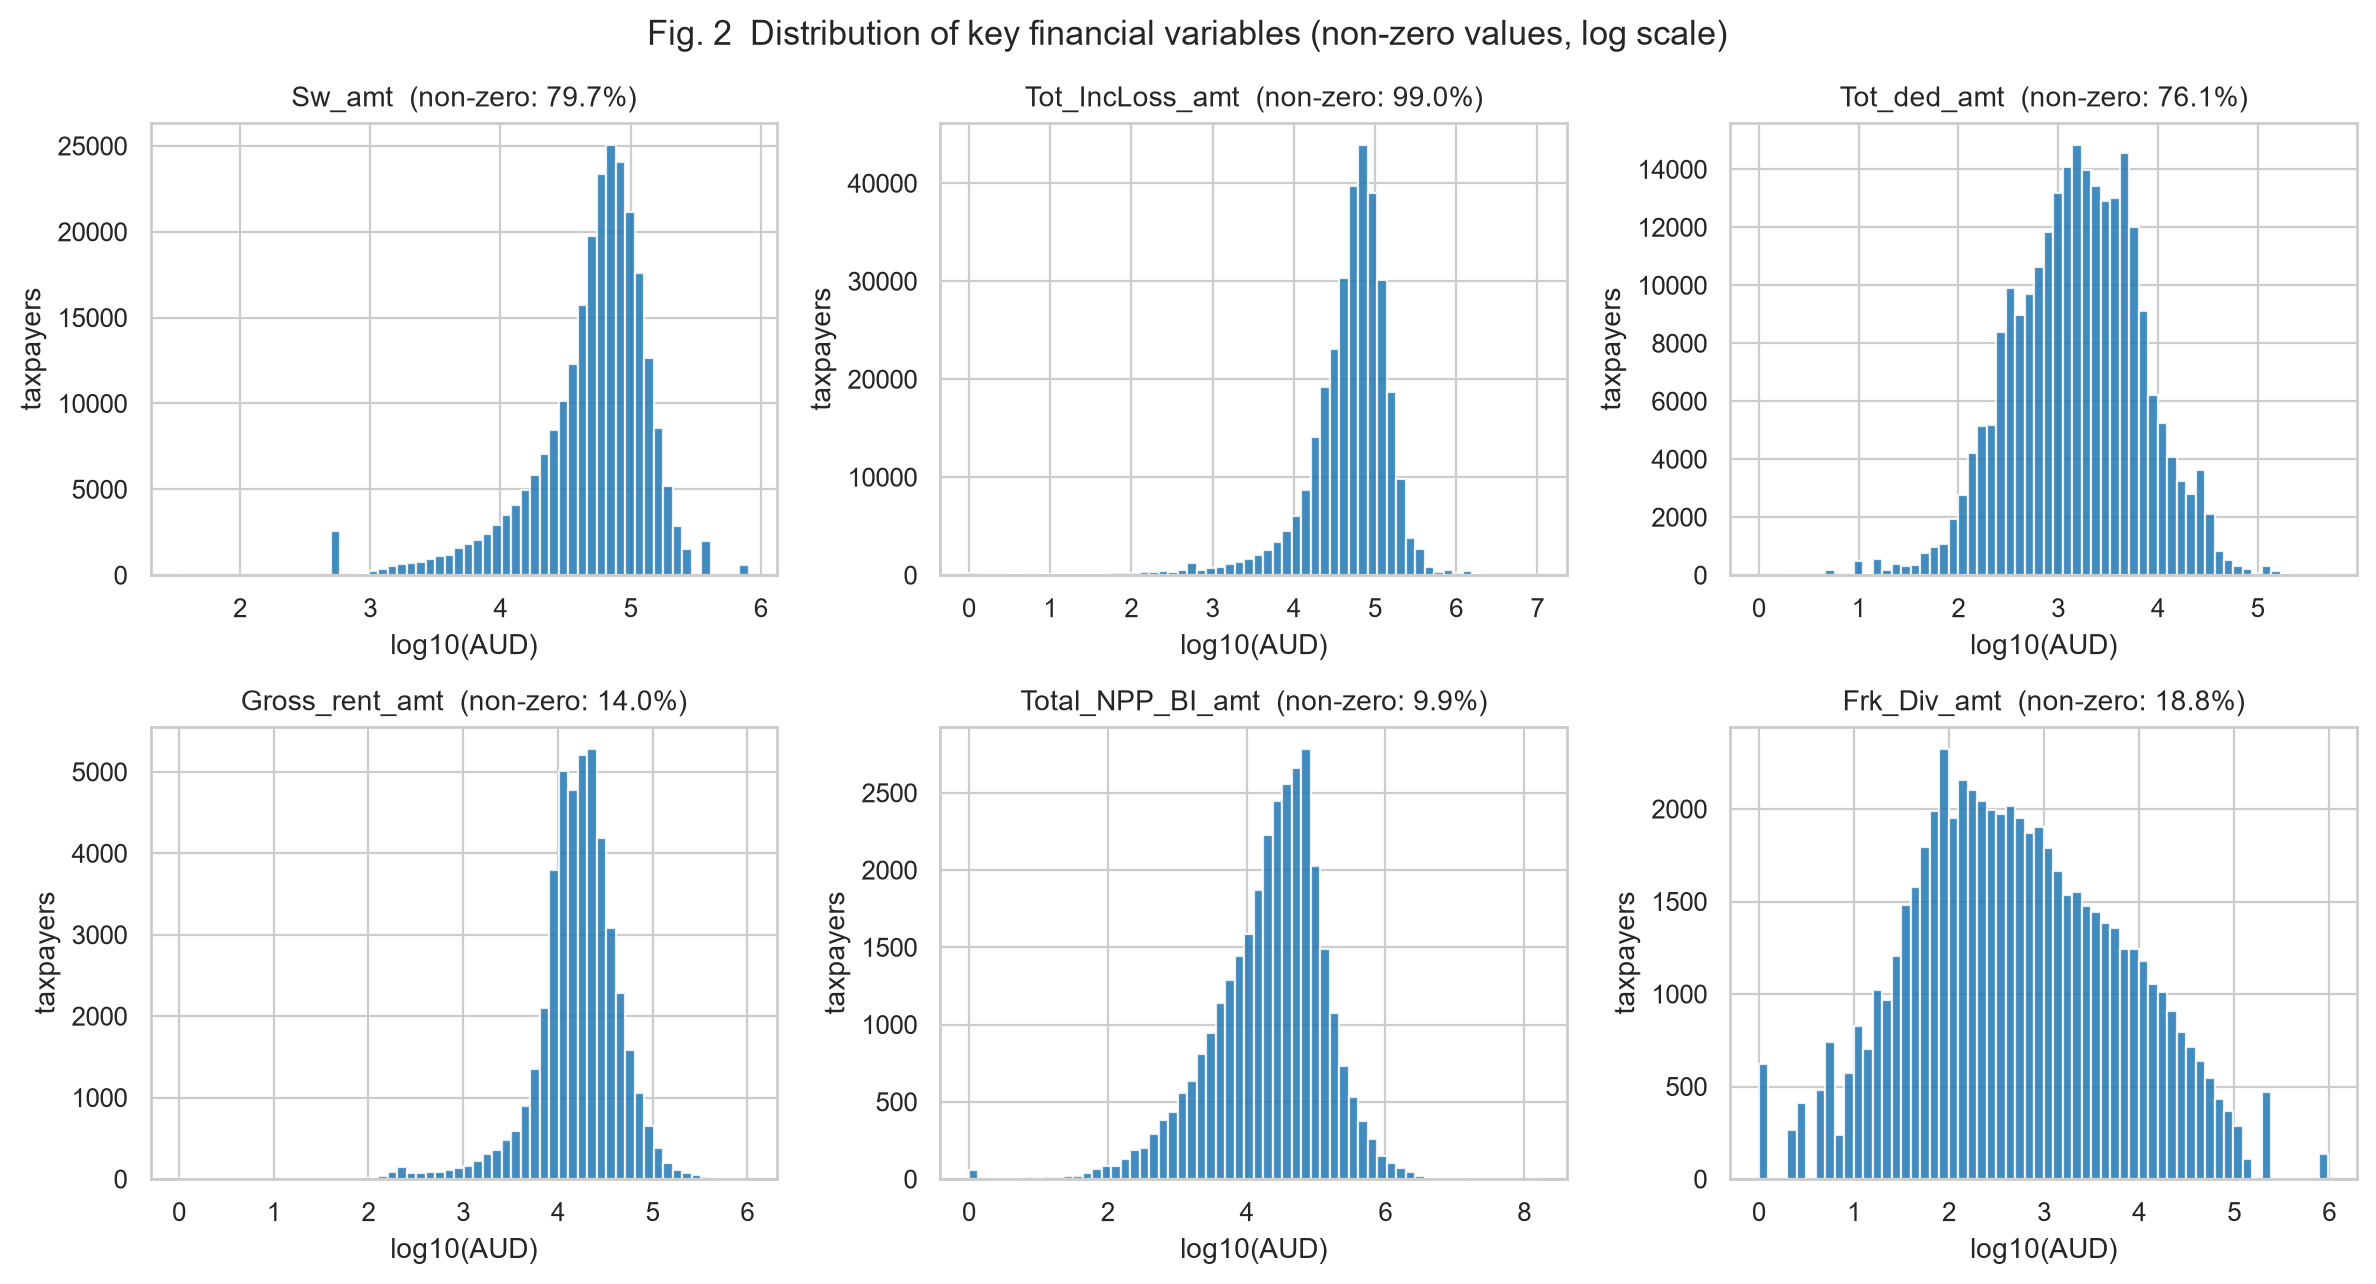
\includegraphics[width=\linewidth]{figures/fig02_variable_distributions.png}
    \caption{Distribution of key financial variables (non-zero values, log scale).}
    \label{fig:distributions}
\end{figure}

\subsection{Preprocessing and Feature Engineering}

Amounts reported by fewer than 1\% of taxpayers were removed (ten variables, e.g.\ primary-production business items), because a variable that is almost always zero would be flagged merely for being non-zero. Of the remainder, one member of each pair with $|r| > 0.95$ on the transformed scale was dropped to avoid double counting: the franking credit ($r = 0.998$ with franked dividends), other rental deductions (0.992 with gross rent) and business expenses (0.951 with business income); their information is retained through ratios. Forty-four amounts remain.

The main dataset included 65 variables including taxpayer characteristics, income items, deductions and etc. In this research, we employed ten financial ratios instead of using the raw variables as relying on raw dollar amounts for anomaly detection could lead to issues where only individuals with significantly high or low incomes, or extreme or low deduction amounts, would be identified as anomalies. Therefore, we utilized these ratios to transform the model's variables into quantifiable and comparable values that can be assessed among taxpayers without concerns about their income levels and provide a standard format for benchmark assessments. The ratio of work-related expenses to salary is applicable for taxpayers earning a salary, while the rental deduction to rental income ratio serves as a means for anomaly detection among those with rental income, and the ratio of business expenses to business income is relevant for individuals with business income.

The 44 transformed amounts are combined with twelve behavioural features (Table~\ref{tab:features}). Each ratio divides by $\max(\text{denominator}, \$1{,}000)$ and is capped, so division by zero cannot occur. The taxable income ratio checks whether the reported taxable income amount matches the calculated amount from other variable including income and deductions.

\begin{table}[H]
    \centering
    \caption{Behavioural features of the research.}
    \label{tab:features}
    \small
    \begin{tabular}{p{0.30\linewidth} p{0.31\linewidth} p{0.30\linewidth}}
        \toprule
        Feature & Definition & Description \\
        \midrule
        deduction\_to\_income\_ratio & total deductions / total income & Could signal over-claiming expenses \\
        wre\_to\_salary\_ratio & five work-related expense items / salary & Benchmarked by occupation \\
        business\_expense\_ratio & business expenses / business income & Could signal over-claiming expenses or unreported income \\
        rental\_deduction\_ratio & three rental deduction items / gross rent & Rental losses lead to potential audit risk \\
        taxable\_income\_ratio & taxable income / (income $-$ deductions $-$ losses) & Internally inconsistent return \\
        investment\_deduction\_ratio & interest and dividend deductions / investment income & Investment deductions without matching income \\
        gift\_to\_income\_ratio & gifts and donations / total income & Very large donation claims compared to income \\
        tax\_affairs\_cost\_ratio & cost of managing tax affairs / total income & Unusually high advisory cost \\
        personal\_super\_ratio & personal super contributions / total income & Contributions far above income are unusual \\
        payg\_instalment\_ratio & PAYG instalment credits / total income & Instalments inconsistent with declared income \\
        items\_reported & number of non-zero amount fields & Return complexity \\
        lodged\_via\_agent & 1 if lodged by a tax agent & Agent-prepared returns claim differently \\
        \bottomrule
    \end{tabular}
\end{table}

\subsection{Segmentation}

The k-means algorithm depends on the value of $k$ and clustering with different $k$ values will eventually produce different results. Candidates for $k$ number were compared using several methods. First we used inertia elbow method, where it measure how internally coherent the clusters are. Second, silhouette method where it shows the separation distance between the resulting clusters~\cite{rousseeuw1987silhouettes}. Third, we used Davies--Bouldin Index as it is calculated as the average similarity of each cluster with a cluster most similar to it~\cite{davies1979cluster}. Cali\'nski--Harabasz Index is a measure of how similar an object is to its own cluster (cohesion) compared to other clusters (separation)~\cite{calinski1974dendrite}. It has computed on a fixed 20,000 record sample because silhouette is quadratic. One segment have to have at minimum 2,000 records to support its own forest. Among these methods, $k$ number with highest silhouette and lowest Davies--Bouldin Index was selected. Segments were named after their correlated median income.

\subsection{Anomaly Detection}

One Isolation Forest (200 trees, subsample 256~\cite{liu2008isolation}) was fitted to each segment with 56 features and used to score anomaly of its own clusters. Scores are reported as the negative of scikit-learn's \texttt{score\_samples} so that higher means it is more isolated from the segment. Since contamination percentage only cut-off the top anomaly at 1\%, 2\%, 5\% and 10\% which taken from segment score quantiles, 2\% has been chosen for this research as it is practical rather than an estimate of the unknown true anomaly rate. A population wide forest with identical settings was fitted for comparison. The designs were checked using on overlap score like Jaccard and Spearman at each budget. A pre-specified test was repeated on both designs on the twelve behavioural ratios alone, to tell the effect of the reference group from the effect of the feature.

\subsection{Supervised Learning}

Random Forest operates by creating multiple decision trees, each trained on a random subset of the data and features. The injected labels with the same 56 features from Isolation Forest has been used to train Random Forest~\cite{breiman2001random} (300 trees, minimum leaf three, balanced-subsample class weights) and a histogram gradient-boosting classifier~\cite{friedman2001greedy,pedregosa2011scikit} (300 iterations, balanced class weights). Data were split into 70 and 30 with stratification. Models were evaluated on the hold out set with accuracy, precision, recall, F1, ROC-AUC, PR-AUC and the confusion matrix at threshold 0.5, and again at the same 2\% review budget as the forests so that the paradigms are compared on equal terms.

\subsection{SHAP Explainability}

SHAP (SHapley Additive exPlanations) calculates a feature's contribution by considering all possible combinations of features and averaging the marginal contributions across these coalitions. A surrogate Random Forest was trained to reproduce the K-Means labels from the nine segmentation features~\cite{craven1995extracting}. SHAP evaluates how much each feature contributes to the final prediction across all possible feature combinations. To identify \textit{why was a taxpayer flagged}, TreeExplainer was applied directly to each segment's Isolation Forest. Tree models make decisions through a series of splits, and SHAP can trace these decision paths to quantify each feature's contribution with mathematical precision. It uses the structure of tree models to compute exact SHAP values efficiently, making it fast and accurate method for explaining predictions. SHAP values were computed for 300 flagged and 300 unflagged taxpayers per segment for global summaries and individually for selected taxpayers for waterfall explanations. All experiments use seed 42 with scikit-learn 1.9 and SHAP 0.52~\cite{pedregosa2011scikit}.
